% Options for packages loaded elsewhere
\PassOptionsToPackage{unicode}{hyperref}
\PassOptionsToPackage{hyphens}{url}
%
\documentclass[
]{book}
\usepackage{amsmath,amssymb}
\usepackage{lmodern}
\usepackage{iftex}
\ifPDFTeX
  \usepackage[T1]{fontenc}
  \usepackage[utf8]{inputenc}
  \usepackage{textcomp} % provide euro and other symbols
\else % if luatex or xetex
  \usepackage{unicode-math}
  \defaultfontfeatures{Scale=MatchLowercase}
  \defaultfontfeatures[\rmfamily]{Ligatures=TeX,Scale=1}
\fi
% Use upquote if available, for straight quotes in verbatim environments
\IfFileExists{upquote.sty}{\usepackage{upquote}}{}
\IfFileExists{microtype.sty}{% use microtype if available
  \usepackage[]{microtype}
  \UseMicrotypeSet[protrusion]{basicmath} % disable protrusion for tt fonts
}{}
\makeatletter
\@ifundefined{KOMAClassName}{% if non-KOMA class
  \IfFileExists{parskip.sty}{%
    \usepackage{parskip}
  }{% else
    \setlength{\parindent}{0pt}
    \setlength{\parskip}{6pt plus 2pt minus 1pt}}
}{% if KOMA class
  \KOMAoptions{parskip=half}}
\makeatother
\usepackage{xcolor}
\usepackage{longtable,booktabs,array}
\usepackage{calc} % for calculating minipage widths
% Correct order of tables after \paragraph or \subparagraph
\usepackage{etoolbox}
\makeatletter
\patchcmd\longtable{\par}{\if@noskipsec\mbox{}\fi\par}{}{}
\makeatother
% Allow footnotes in longtable head/foot
\IfFileExists{footnotehyper.sty}{\usepackage{footnotehyper}}{\usepackage{footnote}}
\makesavenoteenv{longtable}
\usepackage{graphicx}
\makeatletter
\def\maxwidth{\ifdim\Gin@nat@width>\linewidth\linewidth\else\Gin@nat@width\fi}
\def\maxheight{\ifdim\Gin@nat@height>\textheight\textheight\else\Gin@nat@height\fi}
\makeatother
% Scale images if necessary, so that they will not overflow the page
% margins by default, and it is still possible to overwrite the defaults
% using explicit options in \includegraphics[width, height, ...]{}
\setkeys{Gin}{width=\maxwidth,height=\maxheight,keepaspectratio}
% Set default figure placement to htbp
\makeatletter
\def\fps@figure{htbp}
\makeatother
\setlength{\emergencystretch}{3em} % prevent overfull lines
\providecommand{\tightlist}{%
  \setlength{\itemsep}{0pt}\setlength{\parskip}{0pt}}
\setcounter{secnumdepth}{5}
\ifLuaTeX
\usepackage[bidi=basic]{babel}
\else
\usepackage[bidi=default]{babel}
\fi
\babelprovide[main,import]{brazilian}
% get rid of language-specific shorthands (see #6817):
\let\LanguageShortHands\languageshorthands
\def\languageshorthands#1{}
\usepackage{booktabs}
\ifLuaTeX
  \usepackage{selnolig}  % disable illegal ligatures
\fi
\usepackage[]{natbib}
\bibliographystyle{plainnat}
\IfFileExists{bookmark.sty}{\usepackage{bookmark}}{\usepackage{hyperref}}
\IfFileExists{xurl.sty}{\usepackage{xurl}}{} % add URL line breaks if available
\urlstyle{same} % disable monospaced font for URLs
\hypersetup{
  pdftitle={Bookdown de NOME-PRODUTO},
  pdfauthor={Daniel Claudino},
  pdflang={pt-BR},
  hidelinks,
  pdfcreator={LaTeX via pandoc}}

\title{Bookdown de NOME-PRODUTO}
\author{Daniel Claudino}
\date{2022-11-18}

\begin{document}
\maketitle

{
\setcounter{tocdepth}{1}
\tableofcontents
}
\hypertarget{apresentauxe7uxe3o}{%
\chapter{Apresentação}\label{apresentauxe7uxe3o}}

Bookdown dos(as) NOME-DO-PRODUTO

\begin{figure}

{\centering 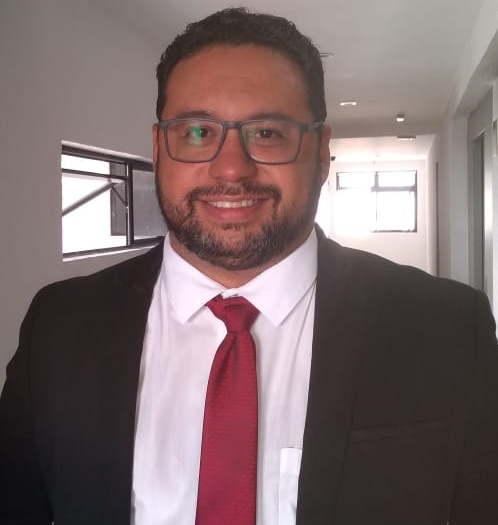
\includegraphics[width=0.5\linewidth]{imagens/FOTO-PERFIL-DANIEL-CLAUDINO-2020} 

}

\caption{Autor}\label{fig:unnamed-chunk-1}
\end{figure}

\begin{itemize}
\tightlist
\item
  Neste bookdown estarão contidos quaisquer \textbf{tipos de produtos} relacionados abaixo. Cada \textbf{tipo de produto} podera estar relacionado a uma ou mais disciplinas, desde o 1º até o 4º ano do curso de Ciência da Computação:

  \begin{itemize}
  \tightlist
  \item
    Notas de Aula
  \item
    Resumos de capítulos de livros;
  \item
    Resumos de apresentações(slides) da disciplina;
  \item
    Minhas apresentações(slides);

    \begin{itemize}
    \tightlist
    \item
      Audience Q\&A (Permite que o público das apresentação envie perguntas para o apresntador)
    \item
      Live Polls (Permite que o público das apresntações realize votações sobre os temas apresentados)
    \item
      Quiz (Permite que o público das apresentações participe de competições integrando-se e assimilando melhor os temas apresentados)
    \end{itemize}
  \item
    Exercícios (elaborados/disponibilizados pelos professores, respondidos ou não em sala);
  \item
    Questionários para as provas;
  \item
    Formulários de pesquisa (Google Forms)

    \begin{itemize}
    \tightlist
    \item
      Elaborados por mim para atendimento de necessidades dos dos meus colegas de sala, dos professores ou da disciplina;
    \end{itemize}
  \item
    Coletas de dados

    \begin{itemize}
    \tightlist
    \item
      Realizadas por mim para atendimento de necessidades dos dos meus colegas de sala, dos professores ou da disciplina; dos dos meus colegas de sala, dos professores ou da disciplina;
    \end{itemize}
  \item
    Planilhas Eletrônicas

    \begin{itemize}
    \tightlist
    \item
      Elaborados por mim para atendimento de necessidades dos dos meus colegas de sala, dos professores ou da disciplina;
    \end{itemize}
  \item
    Filmes, Documentários e outros vídeos

    \begin{itemize}
    \tightlist
    \item
      Recomendados pelos professores, pelos colegas ou por mim;
    \end{itemize}
  \item
    Jogos de aprendizado criados

    \begin{itemize}
    \tightlist
    \item
      (Kahoots / Site principal: kahoot.com / Login do jogador: kahoot.it)
    \end{itemize}
  \item
    Outros materiais elaborados e disponibilizados pelos professores e por mim.
  \end{itemize}
\end{itemize}

Obs: Poderão também ser disponibilizados materiais de outros colegas de curso (com autorização prévia).

\hypertarget{controle-de-versuxe3o}{%
\section{Controle de Versão}\label{controle-de-versuxe3o}}

\begin{longtable}[]{@{}
  >{\raggedright\arraybackslash}p{(\columnwidth - 6\tabcolsep) * \real{0.2500}}
  >{\raggedright\arraybackslash}p{(\columnwidth - 6\tabcolsep) * \real{0.2500}}
  >{\raggedright\arraybackslash}p{(\columnwidth - 6\tabcolsep) * \real{0.2500}}
  >{\raggedright\arraybackslash}p{(\columnwidth - 6\tabcolsep) * \real{0.2500}}@{}}
\toprule()
\begin{minipage}[b]{\linewidth}\raggedright
Versão
\end{minipage} & \begin{minipage}[b]{\linewidth}\raggedright
Data / Hora
\end{minipage} & \begin{minipage}[b]{\linewidth}\raggedright
Colaborador
\end{minipage} & \begin{minipage}[b]{\linewidth}\raggedright
Descrição da Contribuição
\end{minipage} \\
\midrule()
\endhead
0.1 & dd/mm/aaaa xxh00 & \href{https://wa.me/5583988853815}{Daniel Claudino} & Versão inicial do documento \\
\bottomrule()
\end{longtable}

\hypertarget{observauxe7uxe3o-importante}{%
\section{Observação Importante}\label{observauxe7uxe3o-importante}}

\textbf{NOTA}: Este material tem como finalidade auxiliar a fixação de assuntos estudados em sala de aula de acordo com o \textbf{plano de ensino desta disciplina}.

Ele \textbf{não deve ser} utilizado como \textbf{único material de estudo para a prova}, então:

\begin{enumerate}
\def\labelenumi{\arabic{enumi}.}
\tightlist
\item
  Consulte os \textbf{slides da professora} na plataforma FTM;\\
\item
  Faça \textbf{notas de aula} do que for tratado em sala de aula;\\
\item
  Consulte nossas \textbf{notas de aula};
\end{enumerate}

\begin{quote}
\textbf{Dúvidas}: Devem ser encaminhadas no grupo de whatsapp da disciplina.
\end{quote}

\hypertarget{nome-do-produto-da-disciplina-nome-da-disciplina}{%
\chapter{NOME-DO-PRODUTO da Disciplina NOME-DA-DISCIPLINA}\label{nome-do-produto-da-disciplina-nome-da-disciplina}}

Neste capítulo estarão contidos os NOME-DO-PRODUTO da disciplina NOME-DA-DISCIPLINA.

\begin{longtable}[]{@{}ll@{}}
\toprule()
Data & Tópicos Abordados \\
\midrule()
\endhead
dd/mm/aaaa & - Tópico 1- Tópico 2- Tópico 3 \\
\bottomrule()
\end{longtable}

\hypertarget{seuxe7uxe3o-01}{%
\section{Seção 01}\label{seuxe7uxe3o-01}}

\hypertarget{subseuxe7uxe3o-numerada-1}{%
\subsection{Subseção Numerada 1}\label{subseuxe7uxe3o-numerada-1}}

Lorem ipsum. Lorem ipsum. Lorem ipsum. Lorem ipsum. Lorem ipsum. Lorem ipsum. Lorem ipsum. Lorem ipsum. Lorem ipsum. Lorem ipsum. Lorem ipsum. Lorem ipsum. Lorem ipsum. Lorem ipsum. Lorem ipsum. Lorem ipsum. Lorem ipsum. Lorem ipsum. Lorem ipsum.

\hypertarget{subseuxe7uxe3o-numerada-2}{%
\subsection{Subseção Numerada 2}\label{subseuxe7uxe3o-numerada-2}}

Lorem ipsum. Lorem ipsum. Lorem ipsum. Lorem ipsum. Lorem ipsum. Lorem ipsum. Lorem ipsum. Lorem ipsum. Lorem ipsum. Lorem ipsum. Lorem ipsum. Lorem ipsum. Lorem ipsum. Lorem ipsum. Lorem ipsum. Lorem ipsum. Lorem ipsum. Lorem ipsum. Lorem ipsum.

\hypertarget{seuxe7uxe3o-nuxe3o-numerada-3}{%
\subsection*{Seção não Numerada 3}\label{seuxe7uxe3o-nuxe3o-numerada-3}}
\addcontentsline{toc}{subsection}{Seção não Numerada 3}

Lorem ipsum. Lorem ipsum. Lorem ipsum. Lorem ipsum. Lorem ipsum. Lorem ipsum. Lorem ipsum. Lorem ipsum. Lorem ipsum. Lorem ipsum. Lorem ipsum. Lorem ipsum. Lorem ipsum. Lorem ipsum. Lorem ipsum. Lorem ipsum. Lorem ipsum. Lorem ipsum. Lorem ipsum.

\hypertarget{seuxe7uxe3o-02}{%
\section{Seção 02}\label{seuxe7uxe3o-02}}

\hypertarget{subseuxe7uxe3o-numerada-1-1}{%
\subsection{Subseção Numerada 1}\label{subseuxe7uxe3o-numerada-1-1}}

Lorem ipsum. Lorem ipsum. Lorem ipsum. Lorem ipsum. Lorem ipsum. Lorem ipsum. Lorem ipsum. Lorem ipsum. Lorem ipsum. Lorem ipsum. Lorem ipsum. Lorem ipsum. Lorem ipsum. Lorem ipsum. Lorem ipsum. Lorem ipsum. Lorem ipsum. Lorem ipsum. Lorem ipsum.

\hypertarget{subseuxe7uxe3o-numerada-2-1}{%
\subsection{Subseção Numerada 2}\label{subseuxe7uxe3o-numerada-2-1}}

Lorem ipsum. Lorem ipsum. Lorem ipsum. Lorem ipsum. Lorem ipsum. Lorem ipsum. Lorem ipsum. Lorem ipsum. Lorem ipsum. Lorem ipsum. Lorem ipsum. Lorem ipsum. Lorem ipsum. Lorem ipsum. Lorem ipsum. Lorem ipsum. Lorem ipsum. Lorem ipsum. Lorem ipsum.

\hypertarget{seuxe7uxe3o-nuxe3o-numerada-3-1}{%
\subsection*{Seção não Numerada 3}\label{seuxe7uxe3o-nuxe3o-numerada-3-1}}
\addcontentsline{toc}{subsection}{Seção não Numerada 3}

Lorem ipsum. Lorem ipsum. Lorem ipsum. Lorem ipsum. Lorem ipsum. Lorem ipsum. Lorem ipsum. Lorem ipsum. Lorem ipsum. Lorem ipsum. Lorem ipsum. Lorem ipsum. Lorem ipsum. Lorem ipsum. Lorem ipsum. Lorem ipsum. Lorem ipsum. Lorem ipsum. Lorem ipsum.

\hypertarget{nome-do-produto-da-disciplina-nome-da-disciplina-1}{%
\chapter{NOME-DO-PRODUTO da Disciplina NOME-DA-DISCIPLINA}\label{nome-do-produto-da-disciplina-nome-da-disciplina-1}}

Neste capítulo estarão contidos os NOME-DO-PRODUTO da disciplina NOME-DA-DISCIPLINA.

\begin{longtable}[]{@{}ll@{}}
\toprule()
Data & Tópicos Abordados \\
\midrule()
\endhead
dd/mm/aaaa & - Tópico 1- Tópico 2- Tópico 3 \\
\bottomrule()
\end{longtable}

\hypertarget{seuxe7uxe3o-01-1}{%
\section{Seção 01}\label{seuxe7uxe3o-01-1}}

\hypertarget{subseuxe7uxe3o-numerada-1-2}{%
\subsection{Subseção Numerada 1}\label{subseuxe7uxe3o-numerada-1-2}}

Lorem ipsum. Lorem ipsum. Lorem ipsum. Lorem ipsum. Lorem ipsum. Lorem ipsum. Lorem ipsum. Lorem ipsum. Lorem ipsum. Lorem ipsum. Lorem ipsum. Lorem ipsum. Lorem ipsum. Lorem ipsum. Lorem ipsum. Lorem ipsum. Lorem ipsum. Lorem ipsum. Lorem ipsum.

\hypertarget{subseuxe7uxe3o-numerada-2-2}{%
\subsection{Subseção Numerada 2}\label{subseuxe7uxe3o-numerada-2-2}}

Lorem ipsum. Lorem ipsum. Lorem ipsum. Lorem ipsum. Lorem ipsum. Lorem ipsum. Lorem ipsum. Lorem ipsum. Lorem ipsum. Lorem ipsum. Lorem ipsum. Lorem ipsum. Lorem ipsum. Lorem ipsum. Lorem ipsum. Lorem ipsum. Lorem ipsum. Lorem ipsum. Lorem ipsum.

\hypertarget{seuxe7uxe3o-nuxe3o-numerada-3-2}{%
\subsection*{Seção não Numerada 3}\label{seuxe7uxe3o-nuxe3o-numerada-3-2}}
\addcontentsline{toc}{subsection}{Seção não Numerada 3}

Lorem ipsum. Lorem ipsum. Lorem ipsum. Lorem ipsum. Lorem ipsum. Lorem ipsum. Lorem ipsum. Lorem ipsum. Lorem ipsum. Lorem ipsum. Lorem ipsum. Lorem ipsum. Lorem ipsum. Lorem ipsum. Lorem ipsum. Lorem ipsum. Lorem ipsum. Lorem ipsum. Lorem ipsum.

\hypertarget{seuxe7uxe3o-02-1}{%
\section{Seção 02}\label{seuxe7uxe3o-02-1}}

\hypertarget{subseuxe7uxe3o-numerada-1-3}{%
\subsection{Subseção Numerada 1}\label{subseuxe7uxe3o-numerada-1-3}}

Lorem ipsum. Lorem ipsum. Lorem ipsum. Lorem ipsum. Lorem ipsum. Lorem ipsum. Lorem ipsum. Lorem ipsum. Lorem ipsum. Lorem ipsum. Lorem ipsum. Lorem ipsum. Lorem ipsum. Lorem ipsum. Lorem ipsum. Lorem ipsum. Lorem ipsum. Lorem ipsum. Lorem ipsum.

\hypertarget{subseuxe7uxe3o-numerada-2-3}{%
\subsection{Subseção Numerada 2}\label{subseuxe7uxe3o-numerada-2-3}}

Lorem ipsum. Lorem ipsum. Lorem ipsum. Lorem ipsum. Lorem ipsum. Lorem ipsum. Lorem ipsum. Lorem ipsum. Lorem ipsum. Lorem ipsum. Lorem ipsum. Lorem ipsum. Lorem ipsum. Lorem ipsum. Lorem ipsum. Lorem ipsum. Lorem ipsum. Lorem ipsum. Lorem ipsum.

\hypertarget{seuxe7uxe3o-nuxe3o-numerada-3-3}{%
\subsection*{Seção não Numerada 3}\label{seuxe7uxe3o-nuxe3o-numerada-3-3}}
\addcontentsline{toc}{subsection}{Seção não Numerada 3}

Lorem ipsum. Lorem ipsum. Lorem ipsum. Lorem ipsum. Lorem ipsum. Lorem ipsum. Lorem ipsum. Lorem ipsum. Lorem ipsum. Lorem ipsum. Lorem ipsum. Lorem ipsum. Lorem ipsum. Lorem ipsum. Lorem ipsum. Lorem ipsum. Lorem ipsum. Lorem ipsum. Lorem ipsum.

\begin{itemize}
\tightlist
\item
\end{itemize}

  \bibliography{referencias.bib,packages.bib}

\end{document}
